%%%%%%%%%%%%%%%%%%%%%%%%%%%%%%%%%%%%%%%%%
% Stylish Article
% LaTeX Template
% Version 2.1 (1/10/15)
%
% This template has been downloaded from:
% http://www.LaTeXTemplates.com
%
% Original author:
% Mathias Legrand (legrand.mathias@gmail.com) 
% With extensive modifications by:
% Vel (vel@latextemplates.com)
% Final ACS by:
% Juan Barbosa
% License:
% CC BY-NC-SA 3.0 (http://creativecommons.org/licenses/by-nc-sa/3.0/)
%
%%%%%%%%%%%%%%%%%%%%%%%%%%%%%%%%%%%%%%%%%
\documentclass[fleqn,11pt]{SelfArx}
%\usepackage[superscript]{cite}
\usepackage{wrapfig}
\usepackage{rotating}
\usepackage{subcaption}
\usepackage[numbers, super]{natbib}
%----------------------------------------------------------------------------------------
%	ARTICLE INFORMATION
%----------------------------------------------------------------------------------------

\JournalInfo{Laboratorio Org\'anica 3, No. 6, 27/10/2017} % Journal information
\Archive{ }

\PaperTitle{Síntesis de ácidos $\alpha$, $\beta$ - insaturados} %
%\Keywords{Keyword1 --- Keyword2 --- Keyword3} % Keywords - if you don't want any simply remove all the text between the curly brackets
%\newcommand{\keywordname}{Keywords} % Defines the keywords heading name

%----------------------------------------------------------------------------------------
%	ABSTRACT
%----------------------------------------------------------------------------------------

\Abstract{
\begin{wrapfigure}{r}{0.6\textwidth}
	\centering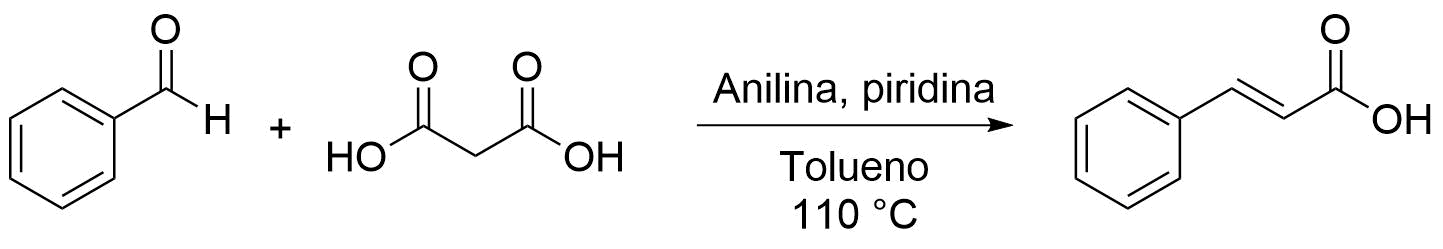
\includegraphics[width=\linewidth]{structures/reaction.png}
\end{wrapfigure}

La preparación del ácido cinámico se llevó a cabo usando benzaldehído y ácido malónico, en tolueno como disolvente. Además se adicionaron piridina y anilina para catalizar la reacción, siendo esta una condensación de Doebner. La reacción tuvo una duración de 18 horas y un rendimiento de 11.6 \%, luego de purificar por recistalización. La caracterización del producto se llevó a cabo usando el punto de fusión el cual fue de 132-13 5$^\circ$C, junto con análisis $^1$HRMN y $^{13}$CRMN, además de un experimento DEPT-135.
}

%----------------------------------------------------------------------------------------

\begin{document}

\flushbottom % Makes all text pages the same height

\maketitle % Print the title and abstract box

%\tableofcontents % Print the contents section

\thispagestyle{empty} % Removes page numbering from the first page
\renewcommand{\tablename}{Tabla} 


%----------------------------------------------------------------------------------------
%	ARTICLE CONTENTS
%----------------------------------------------------------------------------------------

\section*{Introducci\'on} % The \section*{} command stops section numbering
%------------------------------------------------
Las condensaciones de grupos carbonilos se encuentran entre las reacciones más usadas en los mecanismos biológicos para generar grandes moléculas \cite{Wade2013}. Las condensaciones se caracterizan por juntar dos moléculas formando una más grande con la pérdida de una molécula pequeña \cite{Wade2013}. Existe una gran cantidad de condensaciones en la química orgánica, en el caso particular de esta reacción, se usa una modificación de la condensación de Knoevenagel, la cual a su vez corresponde con una condensación aldólica \cite{Palomo2004, List2005}. Sin embargo la condensación de Knoevenagel presenta la ventaja de ser mucho más económica en términos atómicos, dado que la formación de subproductos está limitada, contrario a lo que ocurre con las condensaciones de Wittig y Horner-Wadsworth-Emmons  \cite{List2005}.

El ácido cinámico es un ejemplo de una molécula que es producida metabólicamente por plantas como la canela. Sin embargo esta también tiene un interés sintético, por lo cual dos rutas principales se tienen para obtenerlo, una reacción de Perkin y una condensación de Doebner, siendo la última la que se tratará en el presente documento.

En la reacción de Knoevenagel se produce la adición de un nucleófilo carbonílico sobre un compuesto metileno activado, lo cual genera el aldól, que posteriormente se deshidrara para obtener un compuesto $\alpha,\beta$-insaturado. La modificación de Doebner a la condensación de Knoevenagel consiste en el uso de ácidos carboxílicos como grupos extractores de carga (en el \autoref{sch: knoevenagel}: grupos W). 

\begin{scheme}[h]
	\centering
	\caption{Reacción de Knoevenagel. W: \ce{RCO}, \ce{CO2R}, \ce{CO2NR2}, \ce{RCNR}, \ce{NO2}, \ce{CN}, \ce{SO2R}. R: alquil o aril.}
	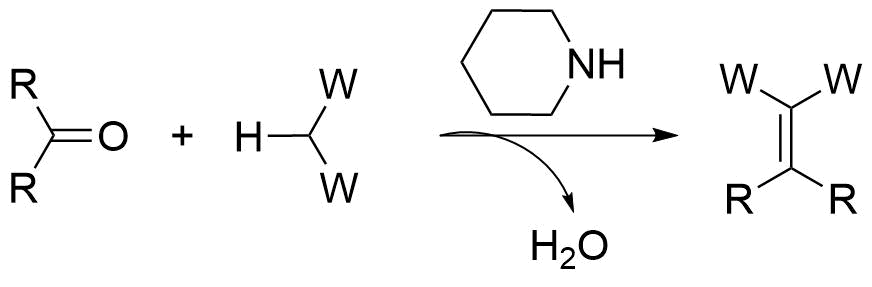
\includegraphics[width=0.8\linewidth]{structures/knoevenagel.png}
	\label{sch: knoevenagel}
\end{scheme}

En la reacción de Doebner el primer paso corresponde con la formación del ion malonato luego de la substracción de un protón del metileno activado, el cual se encuentra estabilizado por resonancia de los carbonilos.
\begin{scheme}[h]
	\centering
	\caption{Obtención del malonato.}
	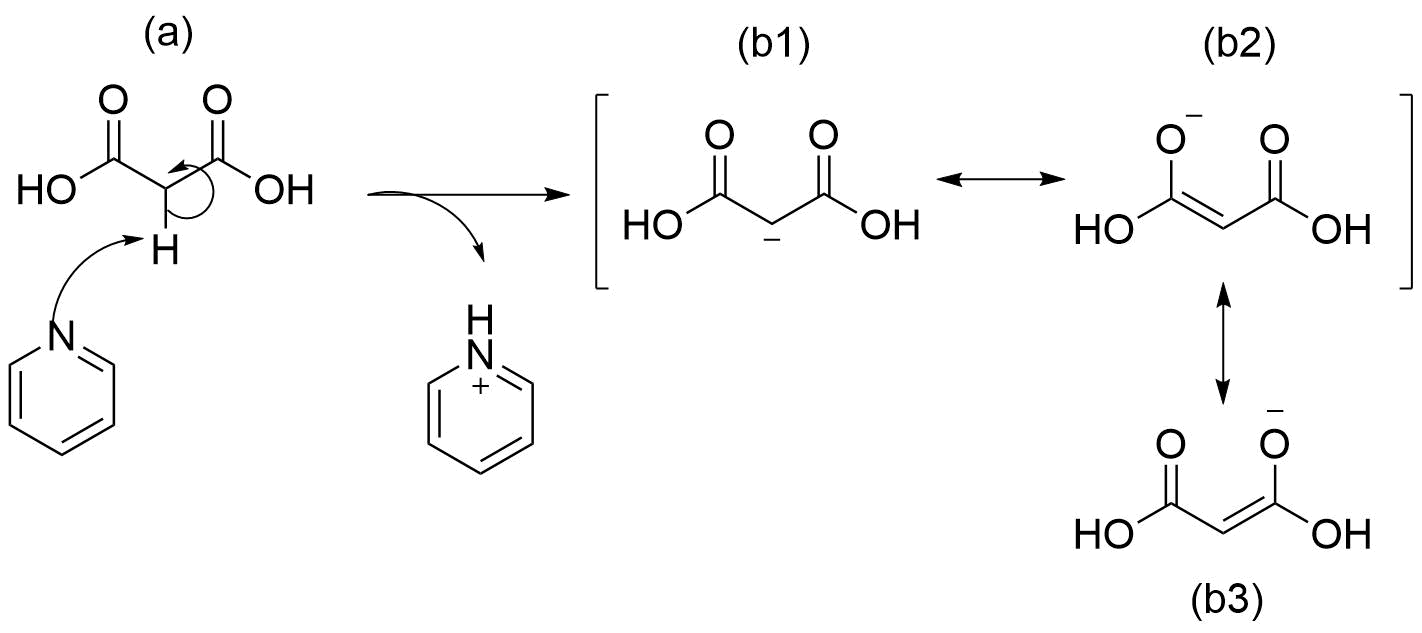
\includegraphics[width=\linewidth]{structures/mechanism1.png}
\end{scheme}

\newpage
Posteriormente tiene lugar el ataque del carbanión sobre el carbono carbonílico del benzaldehído. El cual se muestra en el \autoref{sch: mechanism2}, donde luego del ataque el oxígeno es protonado por un ion piridinio, dando lugar al alcohol. Considerando el carácter básico de la piridina, la misma puede coordinar los protones de los hidroxilos, es de esta forma que se tiene control sobre la estereoquímica de la reacción (\autoref{sch: mechanism3}). El impedimento estérico entre la piridina y el fenilo dan lugar a que se forme únicamente el producto \textit{E}, producto de la rotación de la molécula, lo cual se observa en los pasos (\textbf{f}) y (\textbf{g}).
\begin{scheme}[h]
	\centering
	\caption{Ataque nucleofílico del carbanión.}
	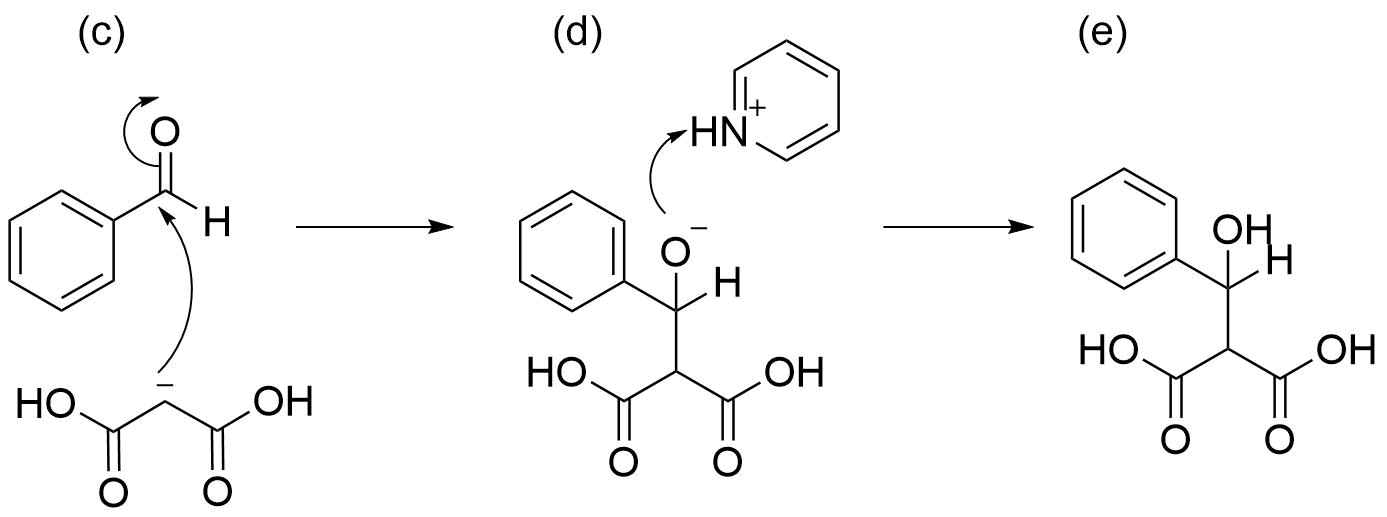
\includegraphics[width=\linewidth]{structures/mechanism2.png}
	\label{sch: mechanism2}
\end{scheme}

\begin{scheme}[h]
	\centering
	\caption{Ataque nucleofílico del carbanión.}
	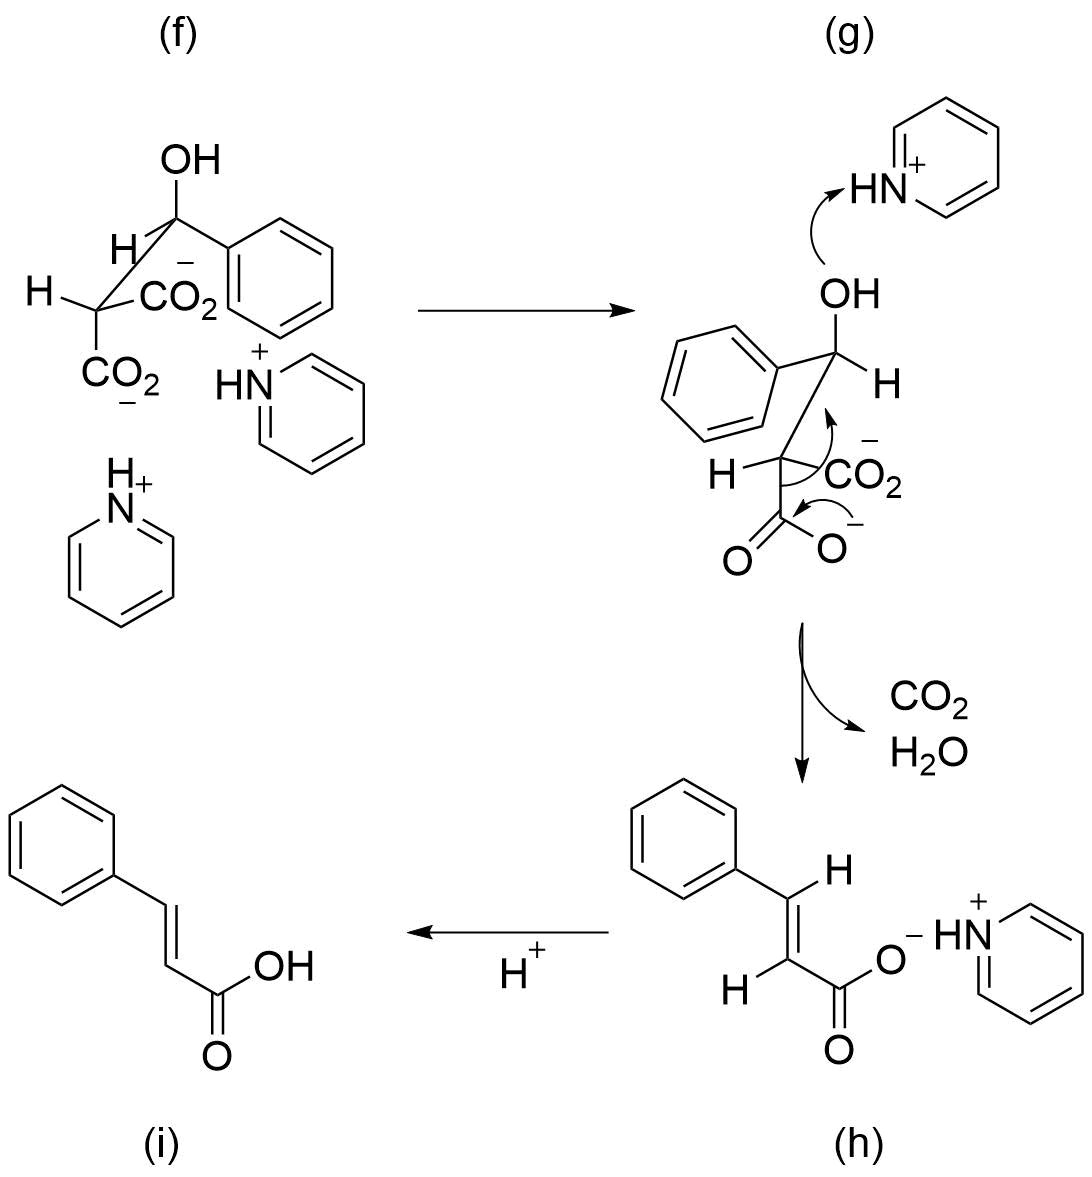
\includegraphics[width=0.9\linewidth]{structures/mechanism3.png}
	\label{sch: mechanism3}
\end{scheme}

Una vez la energía de la molécula se ha minimizado, tiene lugar la descarboxilación, la cual produce dióxido de carbono y agua, además de la regeneración de una molécula de piridina (\textbf{g}). El final de la reacción se da al agregar ácido al médio, el cual regenera el ácido orgánico y libera la piridina al medio.


\section{Resultados y Discusi\'on}
Partiendo con 20.33 mmol de benzaldehído como reactivo limitante se obtuvieron 2.36 mmol de ácido cinámico, correspondientes a un rendimiento del 11.6\% tras recristalizar. El seguimiento de la reacción por CCD mostró la desaparición de la banda correspondiente al benzaldehído (reactivo límite), por lo tanto se esperaba un rendimiento cercano al cuantitativo. El bajo rendimiento calculado se le atribuye a ciertas falencias experimentales asociadas a numerosas transferencias del crudo de reacción al realizar los lavados con bicarbonato y ácido clorhídrico. También se tiene que considerar que la recristalización del producto implica el sacrifico de una considerable cantidad de masa para obtener una mayor pureza. La primera indicación de pureza del producto consistió en la comparación del punto de fusión obtenido con el de la literatura, este se encontraba entre 132-135 $^\circ$C, lo cual concuerda con el consultado. La elucidación de los espectros de RMN $^1$H y $^{13}$C revela que en efecto se obtuvo el producto deseado y que este se encontraba libre de trazas de disolvente o precursores, sin embargo las señales obtenidas indican que el producto se encuentra desprotonado.

El espectro de $^1$H muestra 4 señales correspondientes a los protones ubicados sobre el anillo aromático y aquellos sobre las posiciones vinílicas. Se observa una ausencia de la señal correspondiente al protón del grupo ácido, por lo tanto la suma de las integrales en el espectro indican la presencia de 7 protones en lugar de los 8 esperados. Se plantea la hipótesis de que el espectro obtenido es aquel del anión cinamato, base conjugada del ácido cinámico. Una posible explicación para este resultado implica la presencia de agua en la muestra, causando una desprotonación del ácido cinámico y una consecuente desaparición de la señal del protón ácido. Por otro lado, no se observa la señal correspondiente al agua en \ce{CDCl3}, por lo tanto se plantea la posibilidad de un intercambio del protón con el \_\_\_.

Por otro lado se encuentra un desplazamiento anormal de la señal del protón en posición bencílica, este se encuentra a un desplazamiento de 7.8 ppm, a campo más bajo que los protones aromáticos. Este fenómeno resulta fortuito para soportar la hipótesis de la aparición del anión cinamato en el espectro, en el caso de tener el ácido desprotonado, surgen formas de resonancia para estabilizar la carga sobre el grupo carboxilato que implican una parcial carga positiva sobre la posición bencílica y por ende su desplazamiento a campo bajo.
Otra manera de confirmar esta hipótesis consistió en la comparación del espectro obtenido con los reportados en la literatura tanto para el anión cinamato como para el ácido cinámico. Interesantemente, en el espectro consultado del ácido cinámico, el protón bencílico se encuentra desplazado a campo más alto que en el espectro consultado para el anión cinamato. Esto se explica teniendo en cuenta que el ácido cinámico es neutro y completamente conjugado, por ende la distribución de carga en la molécula no implica una deslocalización de la carga que ubique un carácter positivo sobre la posición bencílica.
Habiendo expuesto estas características peculiares del espectro es posible interpretar de manera más completa las señales obtenidas. En la zona aromática se encuentra una señal en 7.56 ppm que integra para 2 protones, esta se le asigna los protones presentes en posición orto al sustituyente del anillo, por otro lado la señal en 7.42 ppm integra para 3 protones y se asume que en ella se encuentran solapadas las señales de los 2 protones en posición meta y el protón en posición para al sustituyente. Al analizar las señales correspondientes a los protones vinílicos se encuentra la existencia de un efecto techo, causado por el acoplamiento de estos 2 protones a través del doble enlace. La constante de acoplamiento encontrada en estas 2 señales es de $J=16.0$ Hz, lo cual indica que estos protones si se encuentran acoplados y que la geometría del doble enlace es \textit{E}. Este resultado es concordante con la explicación proporcionada en el mecanismo de la reacción para la obtención del alqueno \textit{E}, debido a la organización de la molécula en el estado de transición en el paso de la descarboxilación.

Pasando al análisis del espectro de $^{13}$C, se observa inmediatamente la existencia de las 7 señales esperadas para los átomos de carbono presentes en la molécula. La asignación de la señal de 171.9 ppm resulta trivial y se asocia inmediatamente al carbono del grupo ácido. La señales de las posiciones vinílicas presentan el mismo fenómeno de desplazamiento visualizado en el espectro de 1H, la señal del carbono bencílico se observa a 147.1 ppm, la del otro carbono vinílico a 117.26 ppm, mientras que todas las señales aromáticas se encuentran repartidas entre las señales vinílicas. Para una asignación correcta de las señales aromáticas se analizó el espectro $^{13}$C en paralelo con el espectro $^{13}$C DEPT. Se notificó que en el espectro $^{13}$C DEPT no se evidencia la señal del carbono del grupo ácido debido a que es de carácter cuaternario, también se evidenció que la señal aromática en 134 ppm desaparece en el espectro DEPT, por lo tanto esta se le asigna al carbono ipso a la cadena lateral del anillo. La señal presente en 130.8 ppm se le asigna al carbono en posición para a la cadena lateral, esto se racionalizó por la altura de la señal, que es aproximadamente la mitad de la altura de 2 señales restantes (correspondiente a 2 carbonos cada una, orto y meta). La señal de 128.39 ppm se le asigna a los carbonos en posición meta, mientras que la señal en 128.99 ppm se le asigna a los protones en posición orto, más desprotegidos por la parcial carga positiva presente en la posición bencílica del anillo.

\section{Conclusiones}
Se consiguió sintetizar el ácido cinámico por medio de una condensación de Doebner con benzaldehído, ácido malónico, piridina y anilina. En primera instancia, el punto de fusión medido coincidió con el reportado para el ácido malónico (132-135 $^\circ$C), la verdadera prueba de la obtención del producto se encuentra en los espectros de RMN $^1$H, $^{13}$C y $^{13}$C DEPT. Estos confirman la obtención del producto, sin embargo la distribución de la señales indica que el producto se encontraba desprotonado, lo cual se asocia a un intercambio del protón ácido del producto con el deuterio del \ce{CDCl3}. El rendimiento de la reacción reportado (11.6 \%) no es fiel a la cantidad de producto realmente obtenida, esto se debe al número de pasos involucrados en el tratamiento del crudo de reacción y a la recristalización del producto, por lo tanto se espera que en realidad la reacción haya dado paso a una mayor cantidad de producto que se perdió en estos pasos.
%\pagebreak

\section{Secci\'on experimental}
En un balón de fondo plano fueron mezclados 2.157 g de benzaldehído (20.3 mmol), 2.5 mL de piridina (31.3 mmol) y 0.2 mL de anilina (2.4 mmol), los cuales fueron destilados justo antes de iniciar la reacción., adicionalmente se agregaron al balón de reacción 2.276 g de ácido malónico (21.9 mmol) y 5 mL de tolueno seco. La mezcla se lleva a reflujo por 18 horas. Una vez alcanzado el final de la reacción, se deja enfriar la misma y se adicionan 40 mL de una solución de 10 g de carbonato de potasio. El precipitado se filtra al vacío y se lava sucesivamente con una solución de ácido clorhídrico 3 M y agua. Finalmente es sólido se recristaliza en 10 mL de etanol. 

\paragraph{4-metilacetofenona:}
$^1$H NMR (400 MHz, \ce{CDCl3}) $\delta$ 7.86 (d, J = 8.2 Hz, 2H), 7.26 (d, J = 7.9 Hz, 2H), 2.59 (s, 3H), 2.41 (s, 3H).

$^{13}$C NMR (101 MHz, \ce{CDCl3}) $\delta$ 197.84 (s), 143.87 (s), 134.76 (s), 128.83 (s), 26.58 (s), 21.48 (s).

%----------------------------------------------------------------------------------------
%	REFERENCE LIST
%----------------------------------------------------------------------------------------
%\newpage
\phantomsection
\bibliography{informe}
\bibliographystyle{achemso}

%----------------------------------------------------------------------------------------
\onecolumn
\section{Informaci\'on suplementaria}\label{sec: complementaria}

%\rotatebox{90}
%{
%	\begin{minipage}{0.9\textheight}
%		\centering
%		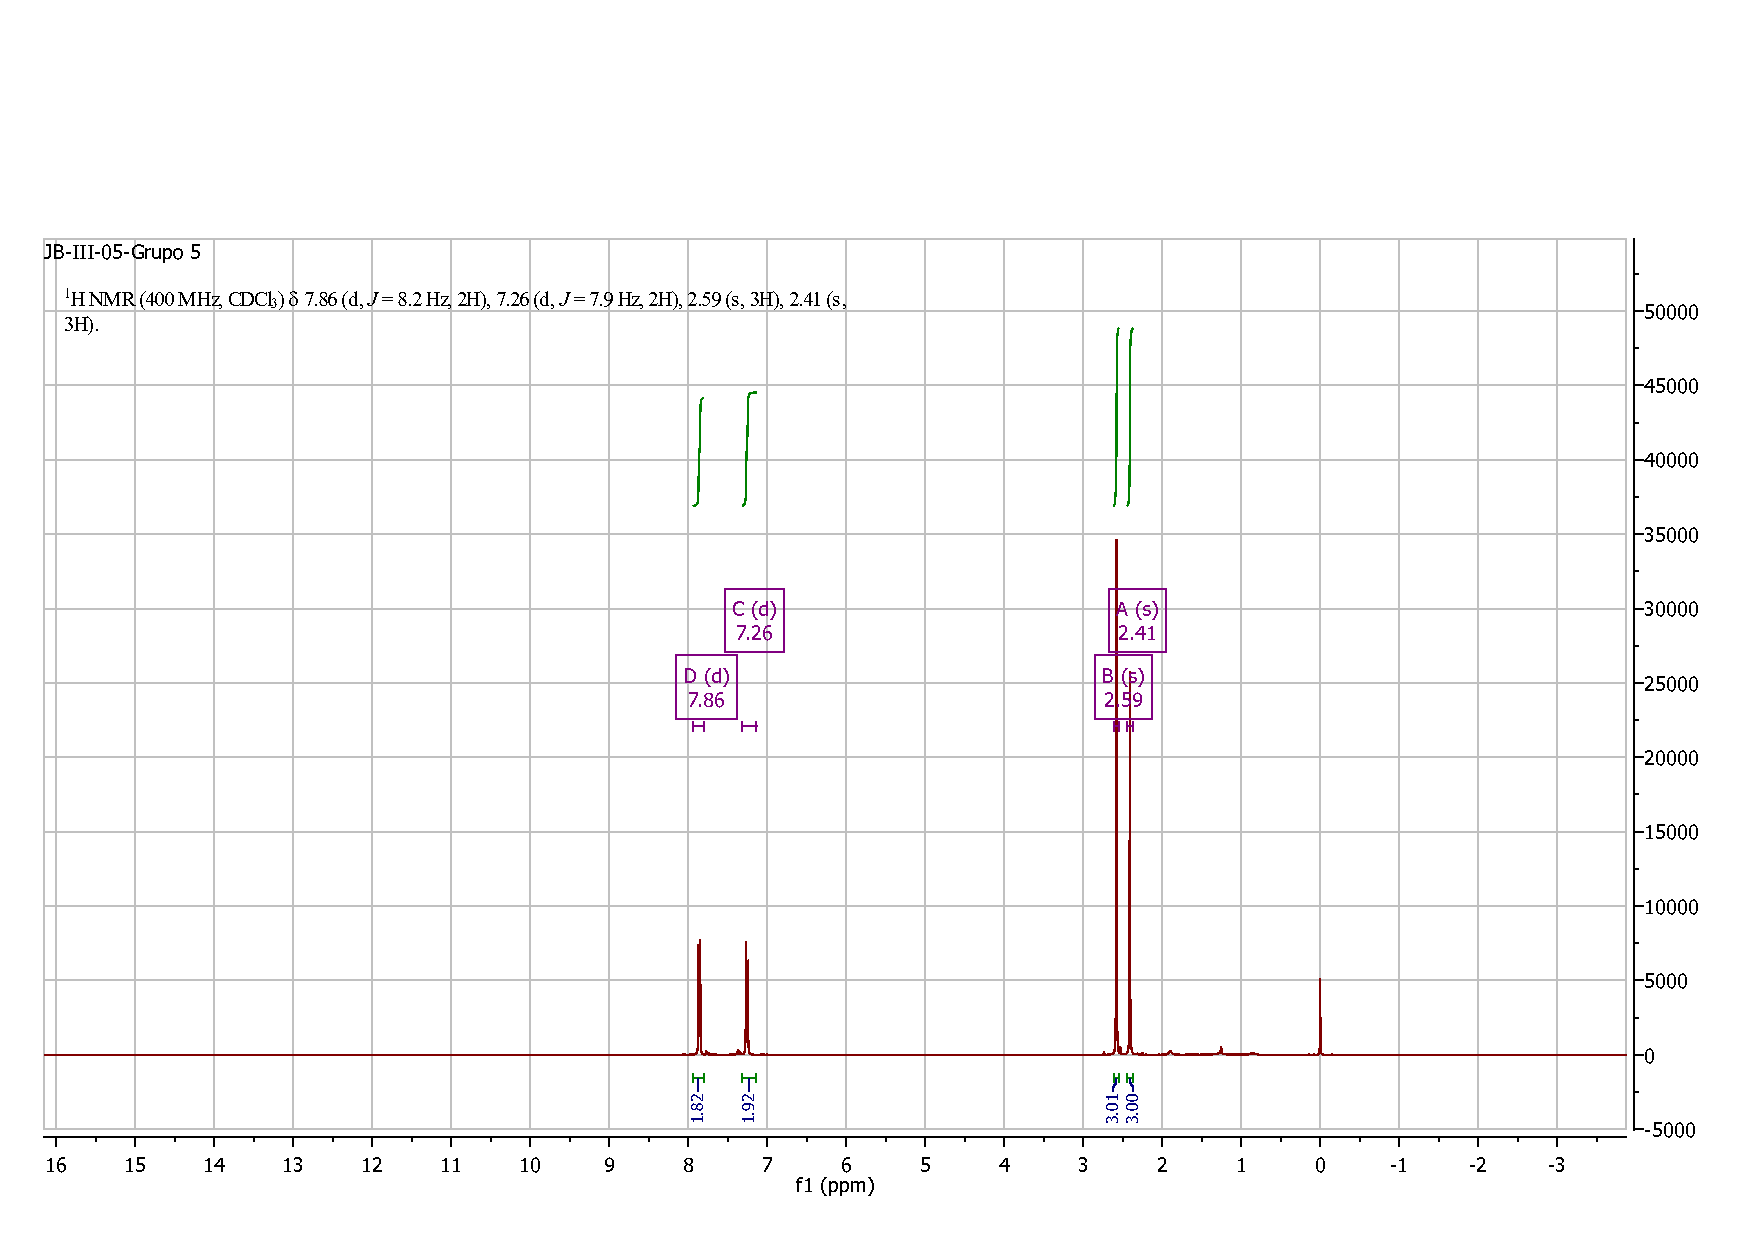
\includegraphics[height=0.7\textheight]{RMN/HRMN.pdf}
%		\captionof{figure}{$^1$HRMN del producto.}
%		\label{HRMN}
%	\end{minipage}
%}
\end{document}